\section{Dimensionality reduction revisited}

\begin{frame}{\secname}

\notesonly{
We want to be able to visualize some data that is high-dimensional. We have already encountered approaches for reducing the dimensionality of the data: PCA is one of them. \figref{fig:spiral} 
provides an example of this.
}

\begin{figure}[ht]
     \centering
     \savebox{\imagebox}{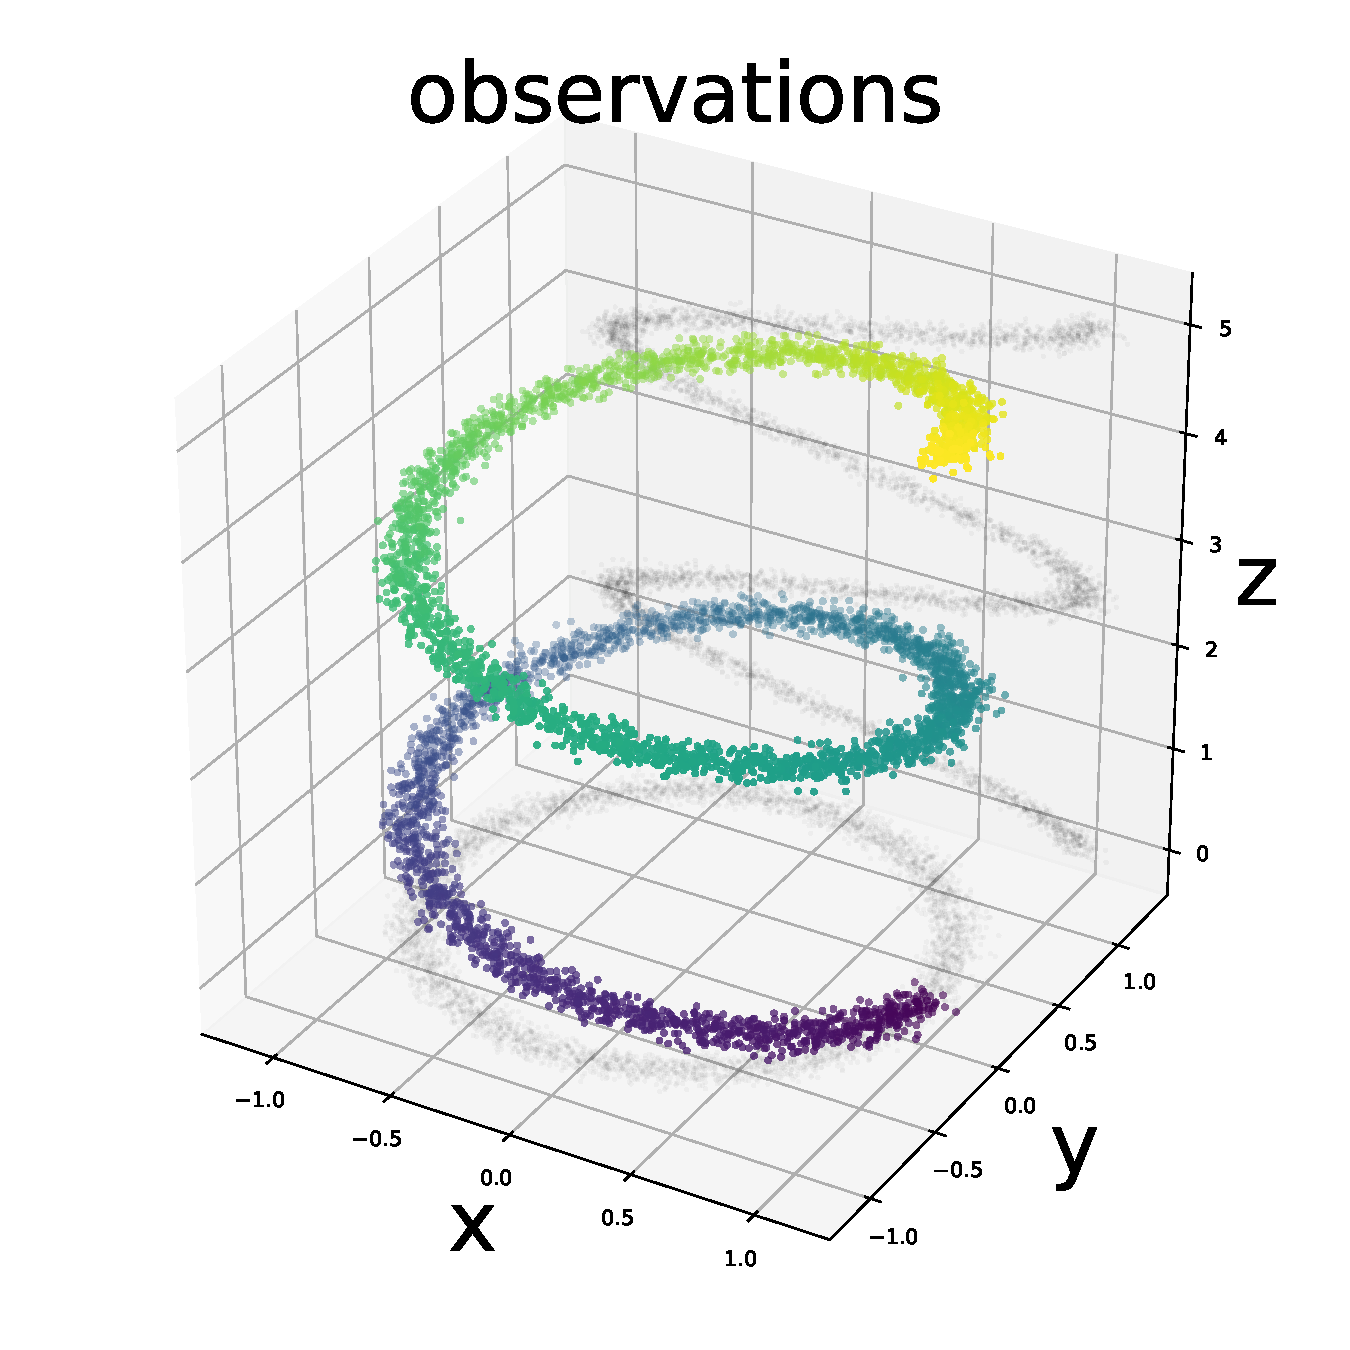
\includegraphics[width=0.4\textwidth]{img/spiral_data}}%
     \begin{subfigure}[t]{0.4\textwidth}
         \centering
         \usebox{\imagebox}% Place largest image
         \caption{original observations}
         \label{fig:spiral_data}
     \end{subfigure}
     \hspace{10mm}
     \begin{subfigure}[t]{0.45\textwidth}
         \centering
         \raisebox{\dimexpr.5\ht\imagebox-.5\height}{% Raise smaller image into place
         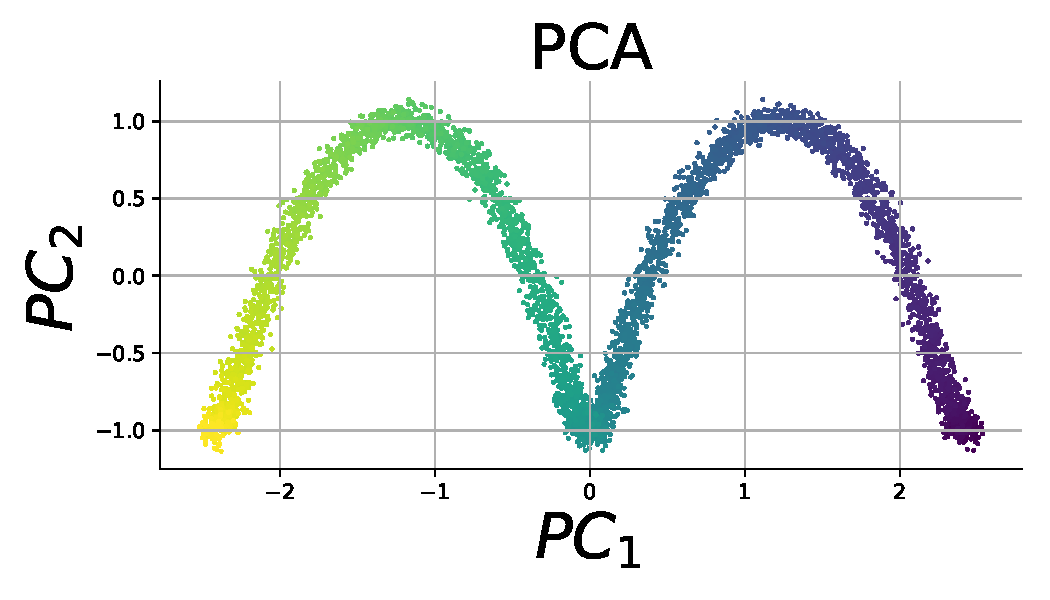
\includegraphics[width=\textwidth]{img/spiral_pca}
         }
         \caption{projection onto the first 2 PCs}
         \label{fig:spiral_pca}
     \end{subfigure}
     \notesonly{\caption{Dimensionality reduction of the spiral data using PCA. Points are colored according to their index in the dataset.}}
	 \label{fig:spiral}
\end{figure}


\end{frame}

\section{Global vs. local structure}

\mode<presentation>{
\begin{frame}
	\begin{center}
	
When determining interesting directions in the data, one will either look for ``global'' or ``local'' structure in this data.

	\end{center}
\end{frame}
}

\subsection{The S dataset}

\begin{frame}{\subsecname}


\notesonly{
Let us examine another dataset on which we will also apply PCA\footnote{We will only consider standard linear PCA.} (c.f. \figref{fig:s_data_pca}). The purpose of this is to make the distinction between global and local structure in the data and which type of structure is captured by PCA (the standard linear version of PCA):
}

\begin{center}
    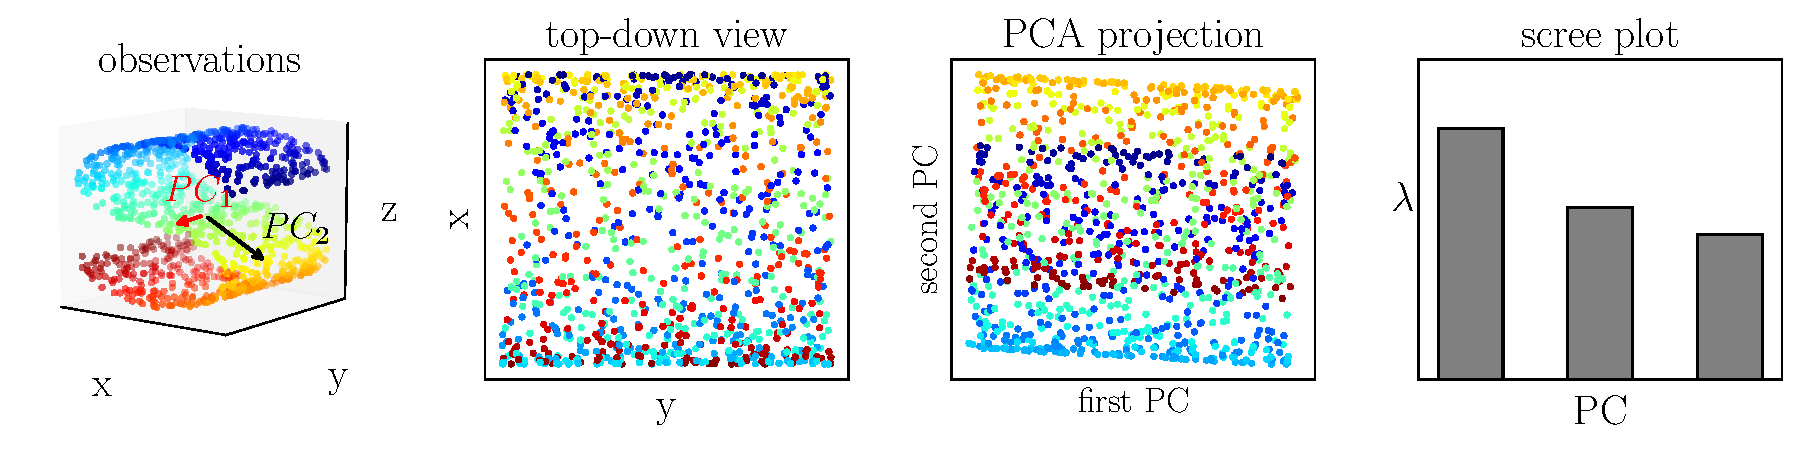
\includegraphics[width=12cm]{img/s_data_pca}
	\captionof{figure}{PCA projection on the ``S'' dataset. Points are colorized according to their index in the dataset.}
	\label{fig:s_data_pca}
\end{center}

\notesonly{
Looking at the PCA projections, we recognize that they closely resemble a top-down view of the data. 
The top-down view is effectively a projection of the data onto the xy-plane. The solution found by PCA is one that explains this 3-dimensional \textbf{S} data using a 2D projection such that the variance explained is maximal. The resemblance between the PCA projections and the top-down view tells us that the main ``directions'' in the data are:
\begin{itemize}
\renewcommand\labelitemi{--}
\item \textbf{First}, the direction explained by the PC with highest eigenvalue ($PC_1$):\\
	A crude way of describing it, is that it lies parallel to the original y-axis. It explains the ``thickness'' of the \textbf{S}.
\item \textbf{Second}, the data also follows the direction of the the original x-axis. It is actually slightly tilted. This tilt explains why some color regions appear more narrow on the $PC_2$ axis, than they do in the top-down view.
\end{itemize}

The scree plot tells us how much variance is explained by each principle component. The difference between the last two PCs is less than the difference between either of them and the first PC. 

\question{Why does $PC_1$ explain more variance than either $PC_2$ or $PC_3$?}\\

- The obvious reason is that this is by design. PCA sorts the PCs in order of descending variance ($\corresponds$ eigenvalues). But this is not what we're asking. The question is specific to this \textbf{S}-data. \emph{Why does the PC that lies parallel to the y-axis explain more variance than the PC that lies parallel to the x-axis?} The reason for this is that any point on the $\textbf{S}$ gets  repeated along the y-axis. This three-dimensional $\textbf{S}$ is really a concatenation of multiple ${S}$-curves. The first PC represents which ${S}$-curve a point belongs to. The only thing left to do is to explain \emph{where} we are on a single curve. The second PC is not sufficient to fully describe this with low reconstruction error. We can only achieve a reconstruction error that is sufficiently low if we also take the third PC into account. So the first thing to point out is that PCA does not give us an ideal dimensionality reduction for this dataset. The slight tilt in $PC_2$ is that it only partially describes the $z$ coordinate of a point. We therefore expect that $PC_3$ is needed to fully recover that $z$ coordinate.
}

\pause 

\question{What is PCA doing wrong on the \textbf{S}-data?}

\notesonly{
- The points were colored according to the order in which they appear in the dataset. PCA does not account for this order. Shuffling the order of the samples leads to the exact same PCs. Nonetheless, we recognize that each group of similarly colored points share proximity to one another. To be more specific: Points with the same color lie on the same location on two different ${S}$-curves. So color represents the position on a curve and that position can only be described by the remaining two PCs. When we look at the PCA projection, we also recognize that colors overlap, specifically Blue, Green and and Red. Those three colors represent different elevation levels on the $\textbf{S}$. \emph{Is this overlap a bad thing?} They have something in common, so we want them to appear closer to one another. So let us look at what the PCA projections tell us about the color groups:


\begin{itemize}
\renewcommand\labelitemi{--}
\item \textcolor{red}{Red} is closer to \textcolor{blue}{Blue} than it is to \colorbox{yellow}{Yellow}. Looking at $PC_2$ confirms this.
\item \textcolor{red}{Red}, \textcolor{blue}{Blue} and \textcolor{green}{Green} are close to one another. Looking at $PC_2$ confirms this also. However, it does not reveal that \textcolor{red}{Red} is actually \textbf{closer} to {\color{green}{Green}}, than it is to \textcolor{blue}{Blue}.
\end{itemize}
}

\notesonly{
What is missing from PCA is that it doesn't prioritize that this $\textbf{S}$ is made up from multiple ${S}$-curves stacked next to each other. Knowing this information enables to find a much more compact representation for describing the data. One might actually find it completely irrelevant that the data describes resembles an $\textbf{S}$ and by doing so, one could find a more compact representation for the data. This is done by finding a representation that focus on preserving local structure.

PCA is designed to find ``global'' structure in the data. It does not restrict itself to preserving local structure. The colors show us the local structure in the data and we no longer recognize this in the PCA projections. Clustering methods base their structure on proximity measures. The proximity can be measured between a point and other data points (e.g. pairwise clustering). Clustering reveals more information about local structure than it does about global structure (i.e. the index/label assigned to a cluster is arbitrary).
}

\end{frame}

\begin{frame}

\slidesonly{
\begin{center}
    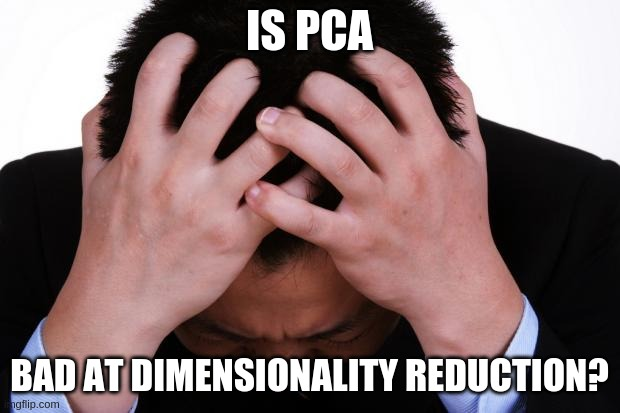
\includegraphics[width=0.5\textwidth]{img/meme_worriedpca}
\end{center}
}

We are not arguing that PCA does a bad job at dimensionality reduction. This is \textbf{not} the takeaway from all this. The point is to that linear PCA attends to global structure and that the user needs to decide whether they are actually interested in global or local structures. Do we care about where we are on an $S$-curve or not?

\end{frame}


%\question{What about ICA?}\\

%- The independence assumption in ICA enables it to find \emph{local} structures.
%Example, applying ICA to face images, yields independent sources sensitive to either the nose nose, mouth or eyes in face.
%On the other hand PCA would find components sensitive to lighting, shape of the face, whole-face expressions (smiling vs. neutral expression) \footnote{see \href{https://scikit-learn.org/stable/auto_examples/decomposition/plot_faces_decomposition.html}{https://scikit-learn.org/stable/auto_examples/decomposition/plot_faces_decomposition.html} for a demonstration.}.



\begin{frame}
\question{What do we mean when we talk about \emph{global} and \emph{local} structures in the data?}\\

\notesonly{
- Pick any two neighboring points from some dataset. Their proximity to one another lets us assume they have more in common than a pair of points that are far away from one another \footnote{This proximity assumption forms the basis for pairwise clustering.}. If we perform PCA on this data and project it onto the principle components, we may find that the two points that were neighbors in the original space are no longer neighbors in the space spanned by the PCs. To be more precise, if their projections do happen to appear close to one another, then this is due to the linearity in the data. But what about non-linear manifolds? PCA does not try to preserve any neighborhood or ``local'' information. This becomes a problem if the ``local'' information is key to \emph{efficiently} reduce the dimensionality.
}

\pause

\begin{figure}[ht]
	\centering
	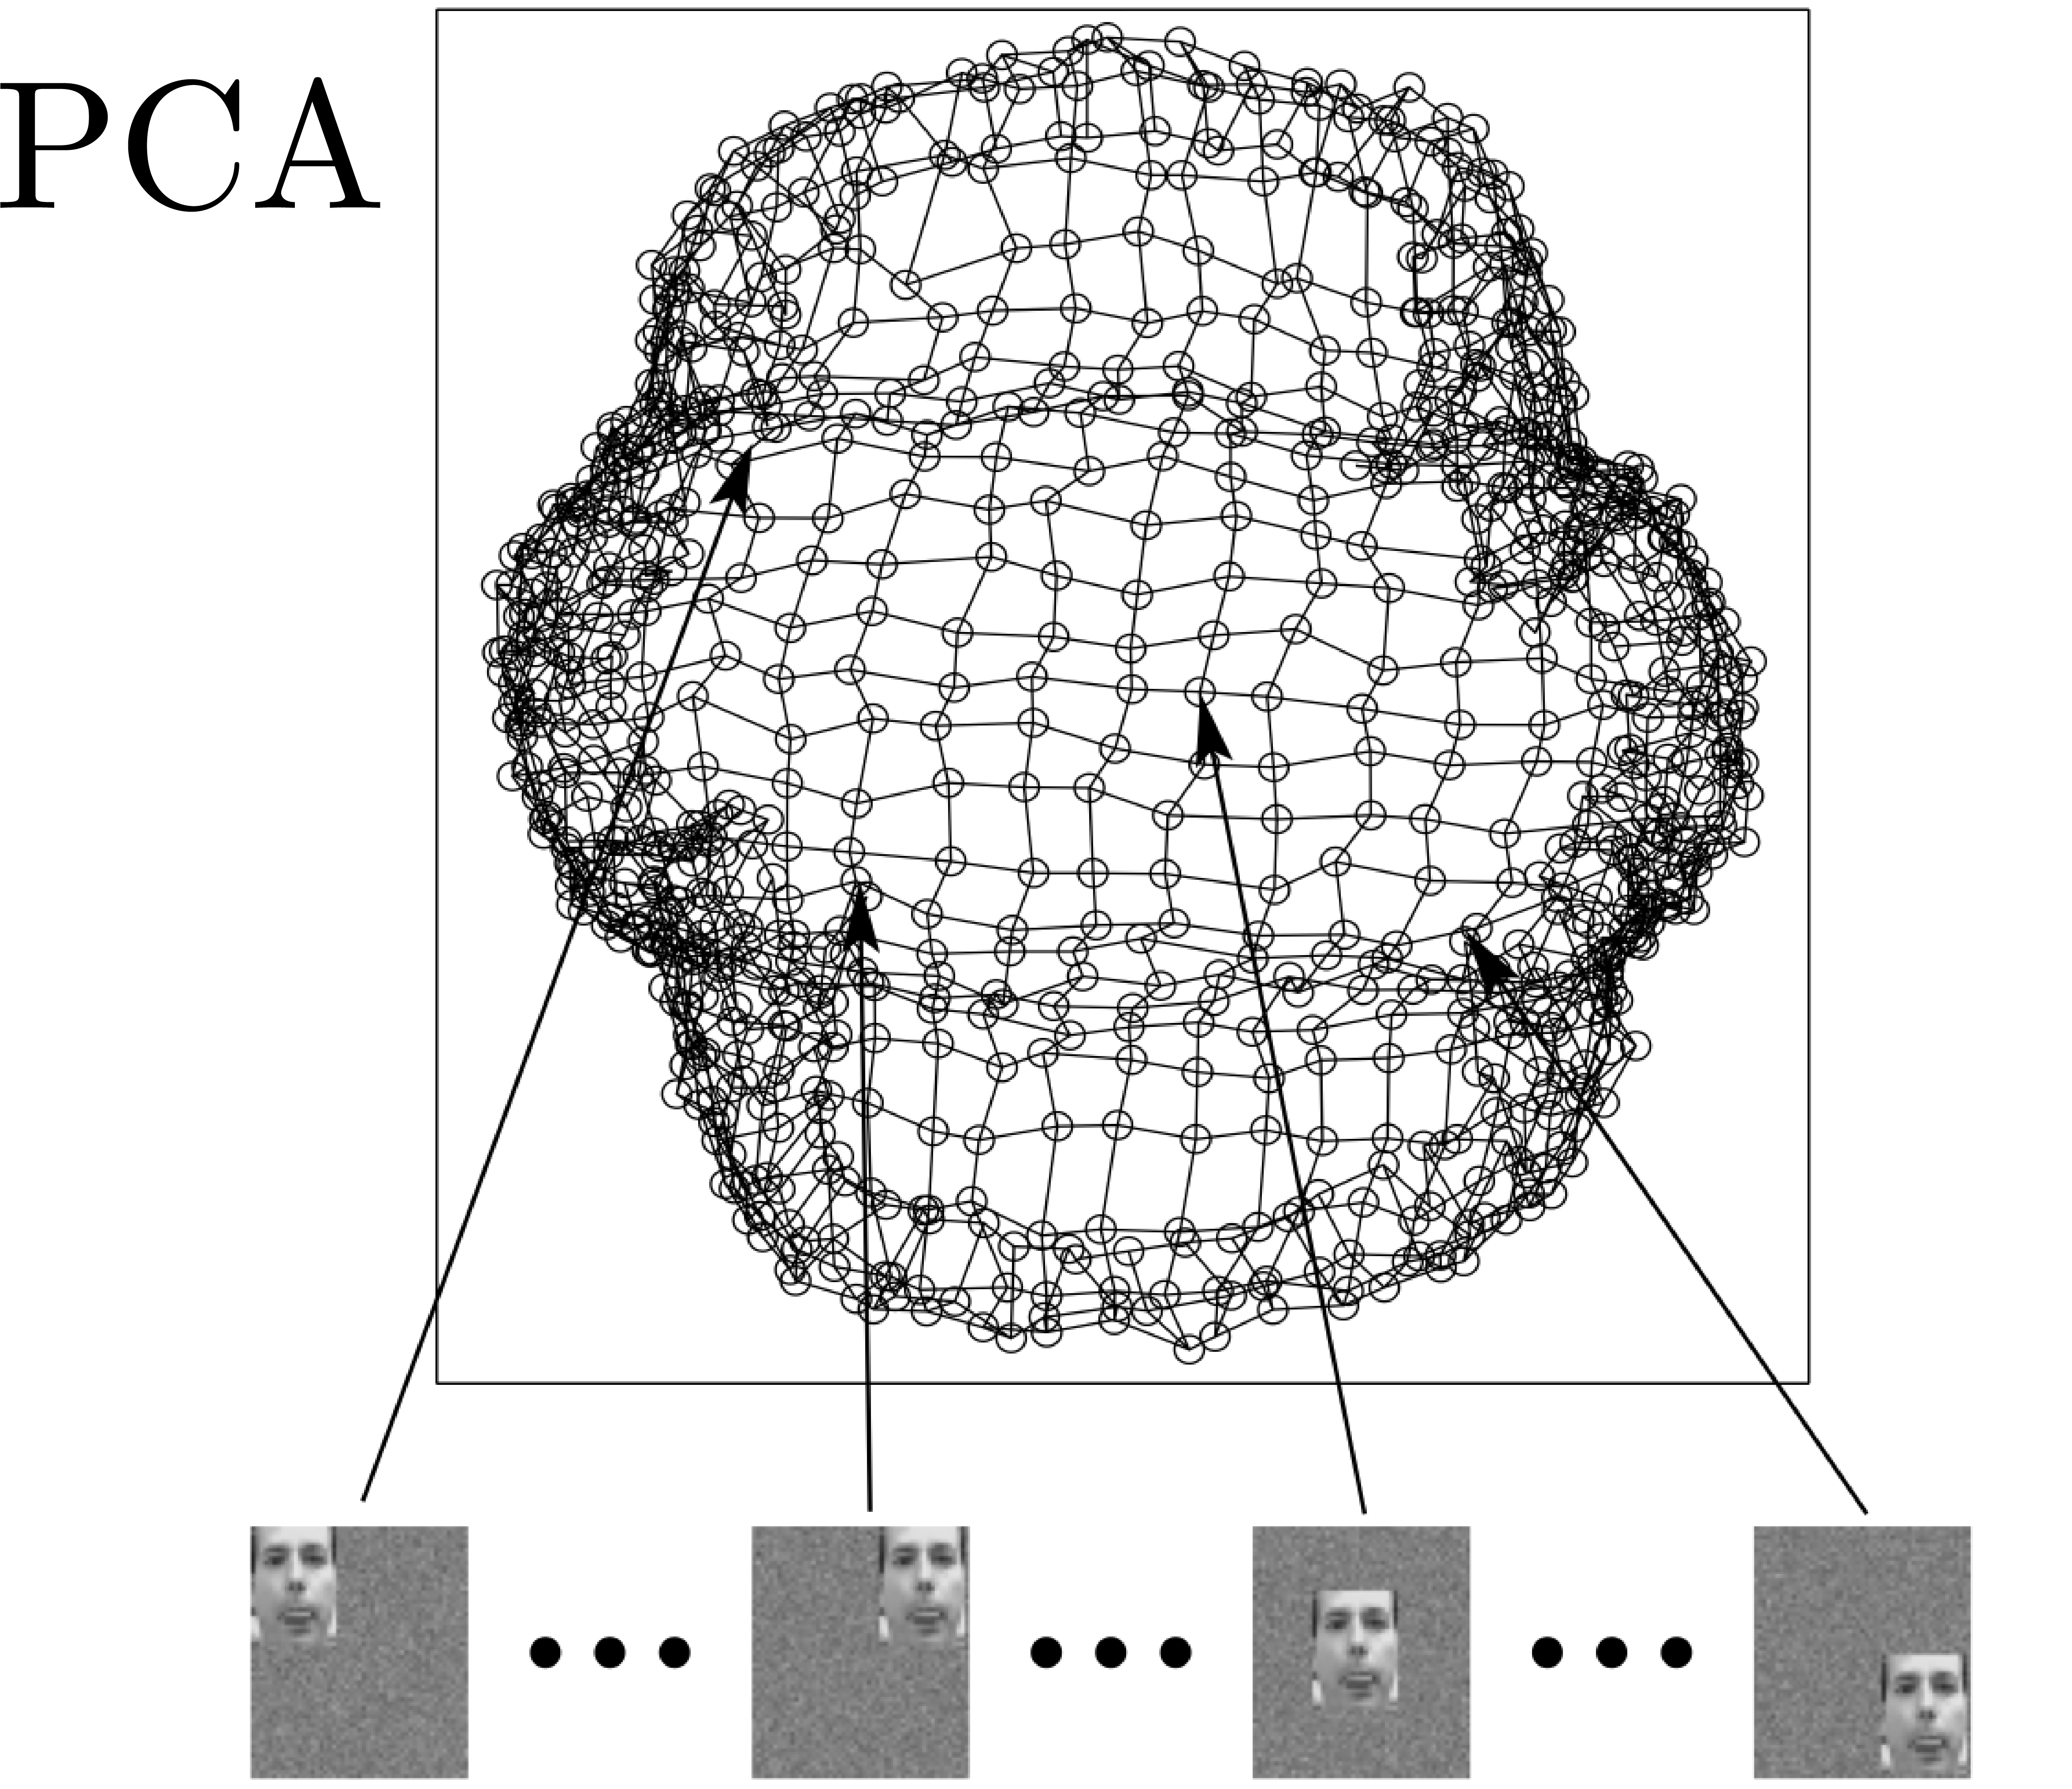
\includegraphics[width=4.3cm]{img/fig3_lle_intro_cropped_pca}
	\caption{PCA projections of translated versions of the same image}
	\label{fig:faces_translated_pca}
\end{figure}

\pause

\question{What are the PC coordinates of an image with the face shifted to the bottom-left corner?}

\end{frame}

\notesonly{
Consider the images in \figref{fig:faces_translated_pca}. The data consists of images where a \textbf{single} picture of a face surrounded by some noisy background. Each image shows the face picture at a different location within the image. The images are projected onto the space spanned by the first two PCs. We examine the projections due to moving the face from one corner to another and find that no relation between the coordinates of the projection and the translation applied to the face picture. If we wanted to predict the coordinates of an image where the face is shifted to the bottom left corner, we wouldn't be able to make that prediction.
}
